\chapter{Dark Matter: Theory and Detection}
It is well established that the majority of the matter in our universe remains undetected. The currently accepted cosmological model (known as the standard cosmological model or \gls{lcdm}) states that the dominant make up of matter in the universe is non-relativistic (cold) and non-baryonic (dark) \cite{wmap9Year}. In this chapter I summarize the argument for cold dark matter (\gls{cdm}), several \gls{cdm} candidates, and some of the prominent past and on going experiments for determination of the cause of \gls{cdm}. 
\section{Missing Mass $\&$ the Case for Dark Matter} 
\subsection{Missing Mass Observations}

\indent The term dark matter (\gls{dm}) as a way of referring to a form of non-luminous matter was first used by Kapteyn \cite{kapteynSidereelAndDM} as a future direction for his studies of stellar dynamics in the disk of the Milky Way. Kapteyn predicted that the distribution of any non-luminous, or dark, matter could be determined by observing the rotation curves of stars in the Milky Way. The issue of missing mass was first observed by Zwicky in 1933 while measuring the red-shifts of galaxies in the Coma cluster (Abell 1656) \cite{zwicky1933redshiftGerman} (English translation: \cite{zwicky1933redshiftEnglish}). His observations found velocities in excess of 2000 km/s for the cluster, which has a luminous mass on the order of 1.6$\times 10^{45}$ g. If the system can be assumed to be in a mechanically steady state, then the virial theorem predicts that:
\begin{equation}
\bar{\epsilon_{k}} = -\frac{1}{2}\bar{\epsilon_{p}},
\label{Eq:virial}
\end{equation}
($\bar{\epsilon_{k}}$ and $\bar{\epsilon_{p}}$ are the kinetic and potential energies). Using Eq. \eqref{Eq:virial} and the observed mass of the luminous matter, the average velocity for galaxies in the cluster would be $\sim$ 80 km/s. This disparity in density (measured by Zwicky to be at least 400 times the density inferred from the stars alone) is the origin of the missing mass problem and the first observational evidence for dark matter.

Following Zwicky's work, little was done to investigate dark matter until galactic dynamics studies of the Andromeda galaxy were done by Rubin and Ford in 1970 \cite{rubinFormM31Curves1970}. They found that the rotation curves did not fit with the virial theorem for the visible matter in the same manner as was observed by Zwicky, reporting a H1 to total mass ratio of between 4 and 8 percent. 


According to Newtonian mechanics the rotation of an orbit should follow:
\begin{equation}
v(r) = \sqrt{\frac{GM(r)}{r}}.
\label{Eq:keplar}
\end{equation}
Crucially, outside the majority of the system's mass, any test mass should have an orbital velocity that drops proportional to $1/\sqrt{r}$; however, this is not observed. The angular velocity of objects around the galactic center remains essentially constant as see in Fig. \ref{Fig:galaxyDispersions}. This observation indicates an increasing mass/luminosity ratio with radius \cite{robertsAndRotsRotationM31M101M81} where previously little matter was believed to exist. Observations of a disparity between luminous matter and a system's rotation curve have been seen in essentially every study for many different galaxies, groups, and clusters with similar results, for example NGC 300 $\&$ M33 \cite{FreemanDisksOfSpiralsAndSos}, NGC 4038/39 \cite{RubinVelCurvesNGC4038and39}, and M81 \cite{robertsAndRotsRotationM31M101M81}. Two conclusions can be drawn from this information: 1) Our theory of gravity is incorrect at these scales, or 2) A large amount of non-relativistic dark matter (\gls{cdm}) is not being accounted for and extends well beyond the baryonic mass in these systems.

\begin{figure}[ht]
\centering
\includegraphics[height = 0.4\paperheight]{rotCurvesNice}
\caption{Rotation curve fit to NGC 6503. The disparity between the measured rotation curve (points), the stellar mass in the disk (dashed line), and the interstellar gas (dotted line) is attributed to an isothermal dark halo (dash-dot line). The sum of these components are the solid fit line \cite{RotationCurvesBegeman1991}. The measured rotation curve is essentially constant with increasing radius past 2 kpc. If the mass were distributed like the visible component, the rotation curve would drop off $\propto 1/\sqrt{r}$ at large radii.}
\label{Fig:galaxyDispersions}
\end{figure}

\clearpage
\subsubsection{\gls{mond} $\&$ the Bullet Cluster}
Modified Newtonian Mechanics (\gls{mond}) postulates that the Newtonian 1/r$^{2}$ relation for gravitating bodies only holds for forces and distances similar to those in the solar system, but that the decline in force with distance is less for weaker forces \cite{Milgrom1983MOND}. \gls{mond} has been used to reproduce the rotation velocities of spiral galaxies without the necessity of additional mass beyond that of the observed baryons and a small neutrino component \cite{MilgromSanders2003MOND}. Work done by Clowe, Gonzalez, and Markevitch in 2004 on mass reconstruction of the interacting cluster 1E0657-558 (the Bullet Cluster) showed that even in a \gls{mond} construction, dark matter of greater mass than the total baryonic contribution was necessary to explain their observations \cite{Clowe2004BulletCluster}.

The Bullet Cluster is an interacting group which has just undergone initial in-fall and pass-through of two different clusters. An x-ray emitting gas has been stripped and separated from the main and sub clusters which are interacting due to the ram-pressure during collision, shown in false colour in Fig. \ref{Fig:bulletCluster}. The galaxies themselves are mainly unaffected in the collision, leaving their gaseous components lagging behind \cite{Stoehr2003DMAnnhilitation}. As the majority of the visible mass in the cluster is found in the gaseous halo, the Bullet Cluster allows for a definitive test of \gls{mond}.

\begin{figure}[ht]
 \centering
 \includegraphics[height = 0.3\paperheight]{bulletCluster}
 \caption{False colour composite image of the interacting cluster 1E0657-558 (the Bullet Cluster). X-ray emissions from the hot interstellar gas (red) accounts for $\sim 80\%$ of the baryonic matter in the cluster. The gas has been stripped from the galactic cores in the collision. The mass in the cluster (blue), measured from micro-lensing studies, is shown to be separated from the x-ray emitting gas, occurring instead around the galactic centres. The mass distribution from the study of this cluster is one of the most definitive arguments for weakly interacting particle dark matter. Composite Credit: x-ray: NASA/CXC/CfA/ M.Markevitch et al.; Lensing Map: NASA/STScI; ESO WFI; Magellan/U.Arizona/ D.Clowe et al. Optical: NASA/STScI; Magellan/U.Arizona/D.Clowe et al. \cite{Clowe2004BulletCluster}}
 \label{Fig:bulletCluster}
\end{figure}
 
If \gls{mond} is correct and all of the mass is of baryonic or neutrino origins, then the mass peak should match the x-ray emission peak (which contains the bulk of the clusters mass). On the other hand, if weakly-interacting \gls{cdm} is the vast majority of the mass, then the peak will be centred around the galactic centres which are separated from the gaseous halos. Mass measurements were done using weak lensing effects, which put the mass peak near the galactic halos. A total mass on the order of $10^{14}$M$_{\odot}$ was found, which is in close agreement to the velocity dispersion measurements made for early-type galaxies by Barrena et al. (2002) \cite{Barrena2002ClusterStudy}. Even under the \gls{mond} model, a non-baryonic mass greater than the that of the baryons is needed, the very problem it was formulated to solve. Thus current formulations of \gls{mond} appear to be excluded.
 

%Why it has to be small well distributed things. Weak lensing backing up research Olsen ref 7 and 8
%\clearpage
\subsection{Cosmic Microwave Background $\&$ $\Lambda$CDM}

Possibly the most convincing argument for the existence of cold dark matter comes from studies of the cosmic microwave background radiation (\gls{cmb}). A widely accepted model for the state of our universe is the \gls{lcdm}, or standard, cosmological model. \gls{lcdm} is fully characterized by six parameters: the age of the universe (t$_0$), the current Hubble parameter ($H_0$), density fluctuations ($\Delta_{R}^2$), the energy densities of baryons ($\epsilon_b$) and cold dark matter ($\epsilon_{CDM}$), and the cosmological constant ($\Lambda$). The model assumes the universe is spatially flat and is dominated by a cosmological constant ($\Lambda$) and cold dark matter (\gls{cdm}). Extensive studies of the cosmic microwave background radiation (\gls{cmb}) by \gls{wmap} \cite{wmap9Year} have found that the model is an adequate fit to the observable \gls{cmb}, large scale structure data, age of globular clusters, observed expansion rates, neutron abundance, and supernovae observations \cite{wmap9Year}. 

The parameter values of the \gls{wmap} study are given in Table. \ref{Table:wmapPerams}. The values of interest to the present study are the \gls{dm} to baryon proportions. The quantity $\Omega_x$ for a species x is defined in terms of its energy density ($\rho_x$) and the critical energy density (i.e. the density at which curvature is zero) of the universe ($\rho_c$) as given by: 

\begin{equation}
\label{Eq:criticalEnergyDensity}
\rho_c \equiv \frac{3H^2}{8 \pi G}
\end{equation}

\begin{equation}
\label{Eq:energyDensity}
\Omega_x  \equiv \frac{\rho_x}{\rho_c}
\end{equation}

These values are important because the expansion rate of the universe is given by the Friedmann equation for scale factor a, curvature k, and Hubble parameter $H$:
\begin{equation}
\label{Eq:friedmann}
\sum\limits_{x} \Omega_x -1 = \frac{k}{H^2 a^2}.
\end{equation}

The curvature value k is one of three values: 0, -1 or 1. The average energy density of the universe determines the curvature, if the density is equal to the critical-density then the universe is spatially flat (k = 0). A subcritical-density universe is negatively curved (k = -1), and a supercritical-density universe is positively curved (k = 1). 

\begin{table}
\centering
\caption{Six parameter \gls{lcdm} fit to the \gls{wmap} nine year data \cite{wmap9Year}.}
\begin{tabular}{l	l	c}
\hline
\hline
Parameter												&	Symbol											&	WMAP Data\\
\hline
Age of Universe (Gyr)									&	t$_0$											& 13.74 $\pm$ 0.11\\
Hubble Parameter (H$_{0}$ = 100h kms$^{-1}$Mpc$^{-1}$)	&	H$_0$											& 70.0 $\pm$ 2.2\\
Baryon Density/Critical Density							&	$\Omega_b$h$^2$									& 0.0463 $\pm$ 0.0024\\
Cold Dark Matter Density/Critical Density				&	$\Omega_c$h$^2$									& 0.233 $\pm$ 0.023\\
Dark Energy Density/Critical Density					&	$\Omega_{\Lambda}$h$^2$							& 0.721 $\pm$ 0.025\\
Curvature Perturbations, k$_0$ = 0.002 Mpc$^{-1}$		&	$10^9 \Delta^2_{\text{R}}$						& 2.41 $\pm$ 0.10\\
\hline
\hline
\end{tabular}
\label{Table:wmapPerams}
\end{table}


\begin{figure}[ht]
\centering
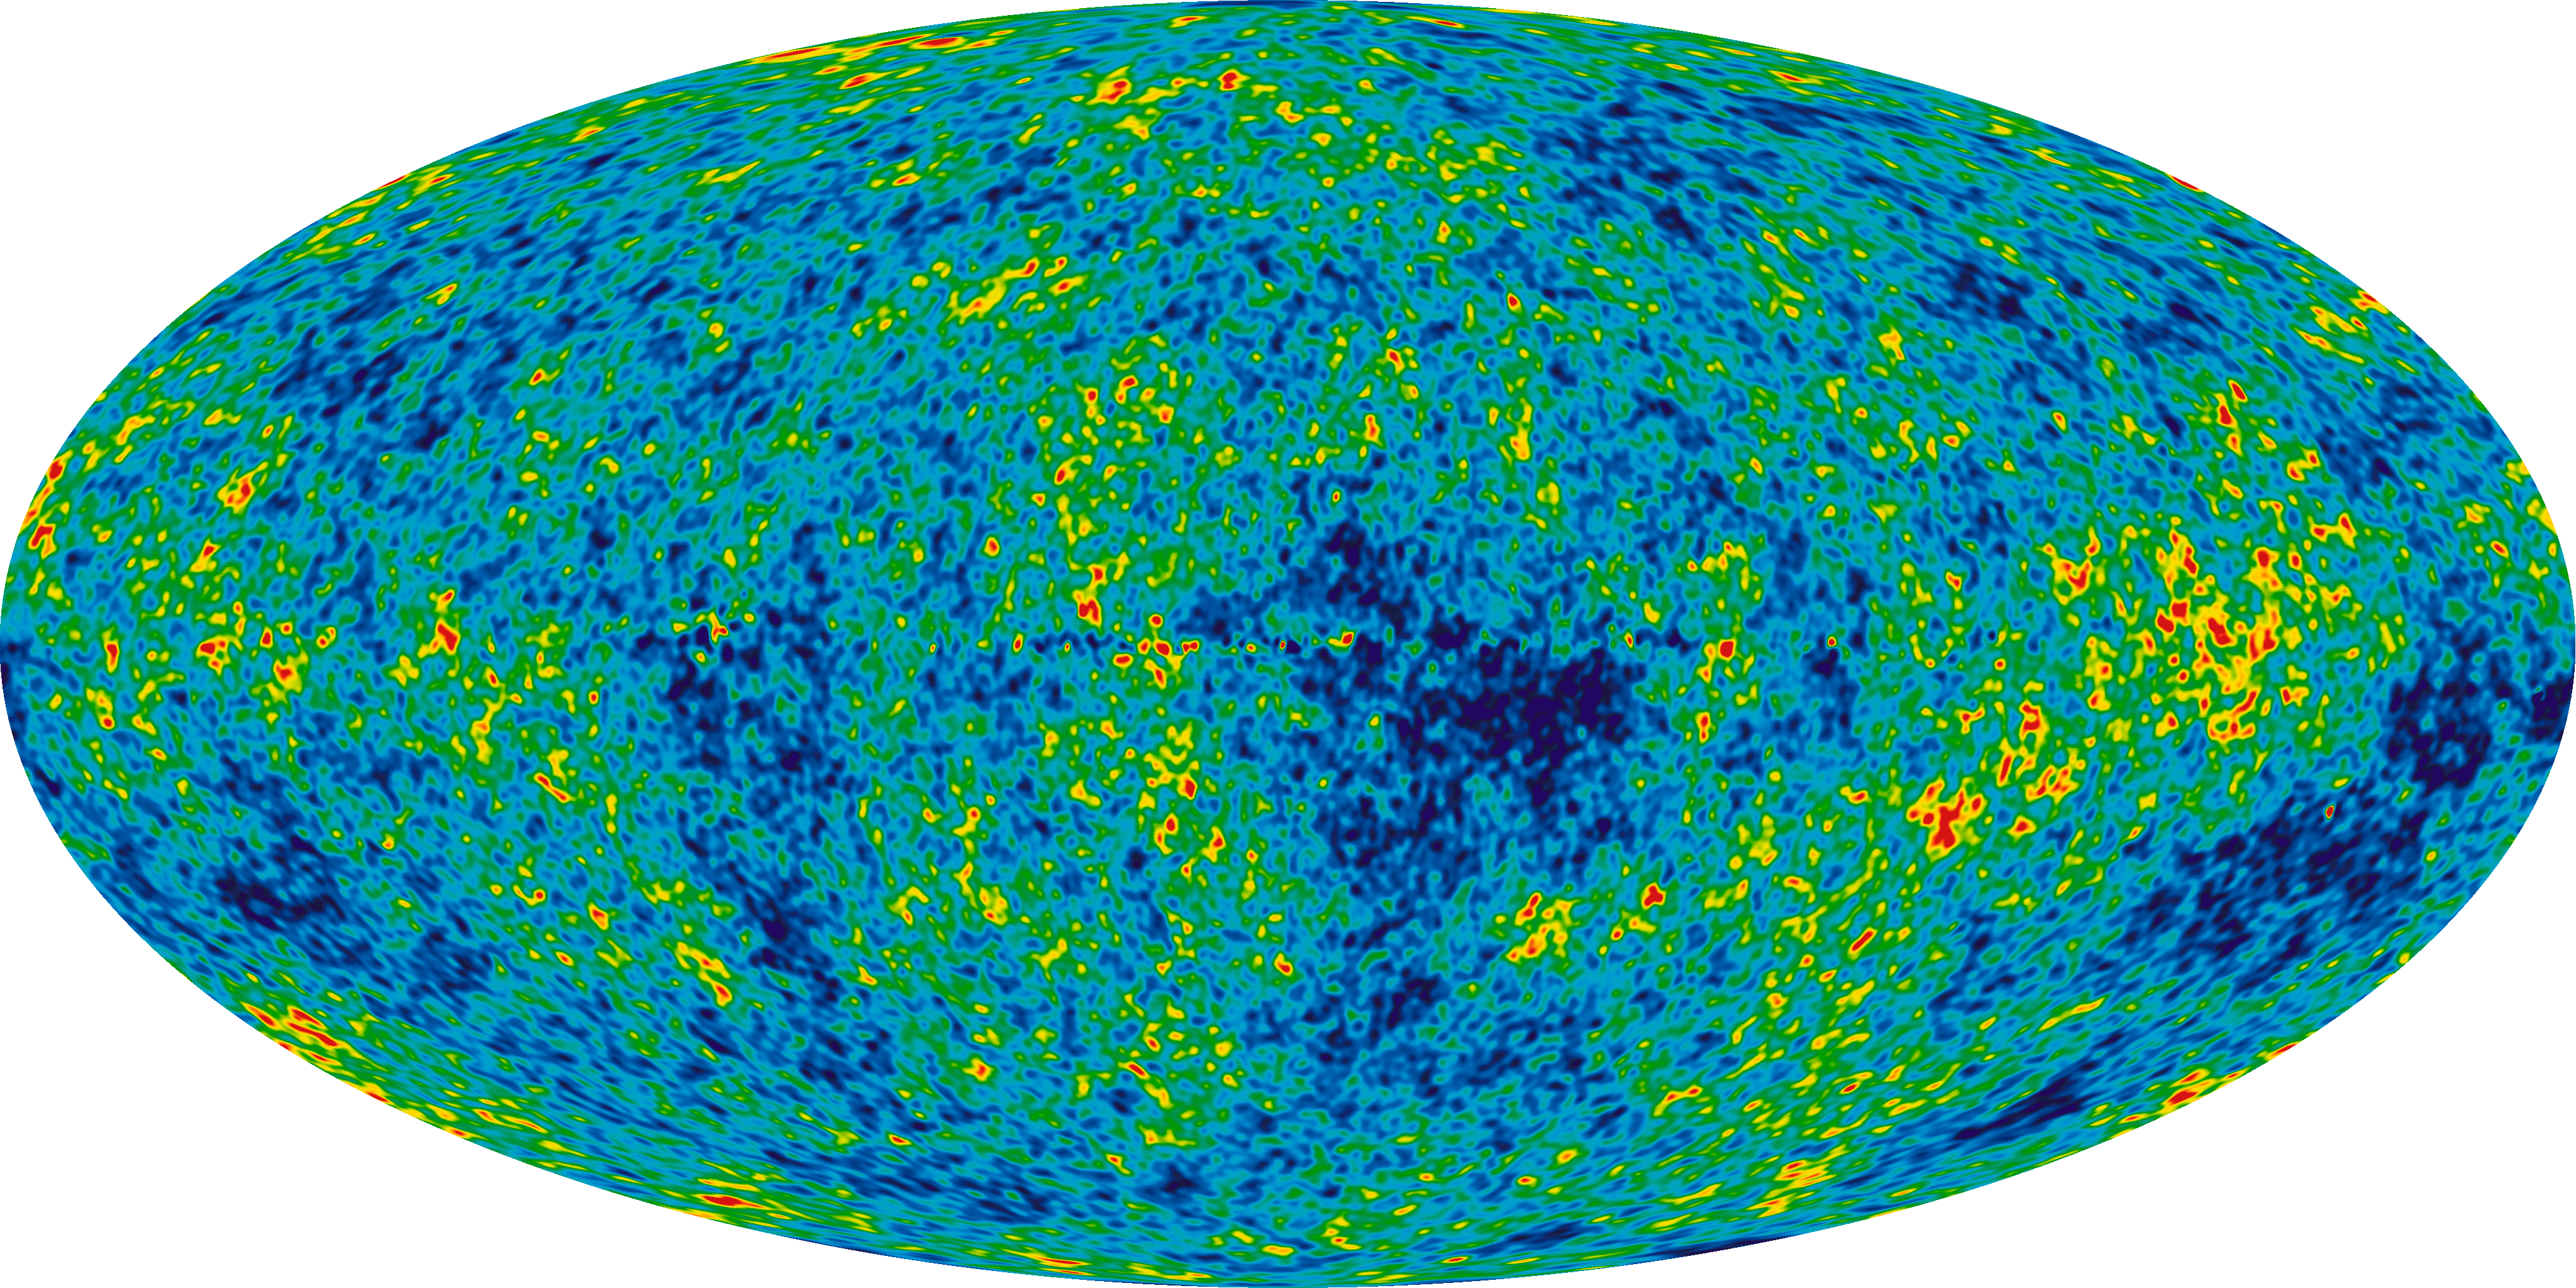
\includegraphics[height = 0.22\paperheight]{WMAP}
\caption{All-sky temperature profile from the nine year \gls{wmap} data release with the Milky Way removed and multipole corrected for our peculiar velocity \cite{wmap9Year}. Fluctuations are shown as color differences corresponding to growth areas of large structures. The temperature range of these fluctuations are within $\pm$ 200 $\mu$K. Credit: NASA / \gls{wmap} Science Team}
\label{Fig:wmap}
\end{figure}

The findings of \gls{wmap} put tight constraints on the characteristics of dark matter. The observations require that there exist particles that interact gravitationally but are chargeless and non-baryonic. Additionally, these particles must be stable or long-lived enough to have survived since the early universe. From the rotation curves discussed above, we infer that dark matter is the dominant constituent of large structures. From the observed clumping it is expected that dark matter must be have been non-relativistic, or cold, at the point of structure formation \cite{wmap9Year}. 

As our galaxy exhibits a rotation curve similar to those of other spiral galaxies, we can conclude that the Milky Way contains a typical amount of \gls{dm} distributed in a similar manner to others \cite{milkyWayRotations}. Therefore, due to dark matter's pervasiveness in our galaxy and the fact that it has yet to be detected, it is assumed to not interact via either the electromagnetic or strong force. Dark matter does, of course, interact gravitationally, and weak interactions have not been ruled out \cite{SMIntro}.


The evidence for a form of cold and non-baryonic dark matter is compelling and well motivated; however it has yet to be detected. Several viable candidates have been introduced and are briefly discussed below. It is important to note that dark matter need not all be of the same species, several may contribute. 

It must be added that there are known species of nonluminous matter that contribute to the observed phenomena. Massive compact halo objects or \gls{macho}s are baryonic masses that were conjectured to exist in galactic halos but to be too faint to be currently observable. Their existence in galactic halos would contribute to the increasing mass-luminosity relations observed in galactic rotation curves \cite{particlDarkMatterReview}. However being baryonic, \gls{macho}s cannot explain all the \gls{wmap} observations.

Another known species of dark matter is the Standard Model (\gls{sm}) neutrino. The neutrino is a lepton, thus non-baryonic, and does not interact electromagnetically or via the strong force. The neutrino, however, is known to have a very small mass, thus is unlikely to make-up a significant portion of dark matter \cite{particlDarkMatterReview}. A larger issue is that neutrinos are relativistic (or hot) and would not explain large scale structure formation \cite{particlDarkMatterReview}. In short, the ideal particle that fits the requirements for \gls{dm} while still being detectable is the family of theorized weakly interacting massive particles (\gls{wimp}s). 


\subsection{Relic Density}
In an expanding universe such as that predicted by the \gls{lcdm} model, a particle species in the early universe would remain in local thermodynamic equilibrium until the expansion rate of the universe (H(t)) exceeded the reaction rate per particle ($\Gamma$) defined as:

\begin{equation}
\Gamma \equiv n \sigma v
\label{Eq:gamma}
\end{equation}
with the particles total annihilation cross section $\sigma$, velocity v, and number density n. Roughly at this equilibrium point, the particle is said to have decoupled or frozen out. Following the argument presented by Bertone, Hooper, and Silk (2004) \cite{particlDarkMatterReview}, the number density of a species $x$ after freeze-out (n$_x$) is determined from the Boltzmann equation and can thus be expressed by:

\begin{equation}
\frac{\text{dn}}{\text{dt}} + \text{3Hn} = -\left< \sigma \text{n} \right> (\text{n}^2-(\text{n}^{\text{eq}})^2),
\label{Eq:numDensityRelics}
\end{equation}
where the number density at thermal equilibrium is n$^{eq}$ \cite{particlDarkMatterReview}. For particles in the non-relativistic limit such as \gls{wimp}s, this can be expressed for particle mass m at temperature T with g degrees of freedom as given by:

\begin{equation}
\label{Eq:numDensityRelicsApprox}
\text{n}^{\text{eq}} = g\left(\frac{\text{m} \text{T}}{2 \pi}\right)^{3/2} \text{e}^{-\text{m/T}}.
\end{equation}

Expanding $\left< \sigma v\right>$ in powers of v$^2$, in terms of constants a and b expressed in GeV$^{-2}$, gives:
\begin{equation}
\label{Eq:annihilCrossSectionThermal}
\left< \sigma v\right> = a + b\left<v^2\right>\frac{T}{m} + \textit{O}{(\left<v^4\right>)}.
\end{equation}

The general relic density for a particle species $x$ can then be expressed in the non-relativistic, low temperature limit as:

\begin{equation}
\label{Eq:genRelicDensity}
\Omega_x h^2 \approx \frac{1.07 \time 10^9 GeV^{-1}}{M_{PI}} \frac{m}{T_F\sqrt{g_*}} \frac{1}{a + 3b \frac{T_F}{m}},
\end{equation}
with g$_*$ as the number of relativistic degrees of freedom evaluated at the freeze-out temperature (T$_F$) for a particle mass m. h is the dimensionless Hubble parameter, h $\equiv \text{H}_0/100$ km s$^{-1}$ Mpc$^{-1}$. An order-of-magnitude approximation to Eq. \eqref{Eq:genRelicDensity} is often useful and is given by:
\begin{equation}
\label{Eq:genRelicDensityApprox}
\Omega_x h^2 \approx \frac{3 \times 10^{-27} \ \text{cm}^{3} \ \text{s}^{-1}}{\left< \sigma v \right>} \approx \frac{m n_x}{\rho_c}.
\end{equation}

A viable \gls{wimp} candidate should have a relic density that is constrained near that predicted by \gls{wmap}, which serves as a useful sanity check for a suggested theory. 


%\clearpage
\section{WIMP Candidates}
The Standard Model of particle physics (\gls{sm}) is known to be an incomplete theory. For one example, it does not yet include neutrino oscillations \cite{SMIntro}. There are numerous theorized extensions to the \gls{sm} that include possible \gls{wimp}s including axions, \gls{wimp}zillas, neutralinos, sterile neutrinos, Kaluza-Klein states, and many others \cite{particlDarkMatterReview}. The leading candidate categories are discussed in the following.


\subsection{Extra Dimensional States}
The inclusion of extra spatial dimensions as a way to unify gravity and the electromagnetic forces was introduced mainly through the work of Kaluza in 1921 \cite{kaluza1921unitatsproblem} with his classical extensions to general relativity followed by the inclusion of quantum theory by Klein in 1926 \cite{kleinStates}. Kaluza-Klein (\gls{kk}) states (standing waves) exist as a series (or tower) of different masses determined by their mode number (n) and the radius of the spacial dimension (R) given by the series (in natural units):

\begin{equation}
\label{Eq:kkTower}
m_n = \frac{n}{R}.
\end{equation}
Each state in this series has the same quantum number, color, and charge. The first state is the lightest \gls{kk} particle (\gls{lkp}) and is predicted to have an annihilation cross section of $\sigma v \approx \frac{0.6 \text{pb}}{m^2_{B^{(1)}}[TeV]}$ which is large enough to be within the possible sensitivity of tonne scale detectors such as \gls{deap3} \cite{SMIntro}\cite{particlDarkMatterReview}.


\subsection{Axions}
Charge-parity (\gls{cp}) conservation is observed in quantum chromodynamics (\gls{qcd}). This is an issue as there exists in the \gls{qcd} Lagrangian a \gls{cp} violating term; this disconnect between the theory of \gls{qcd} and experimental results is known as the strong \gls{cp} problem \cite{SMIntro}. Introducing a scalar field to the problem (the Peccei-Quinn mechanism) is a credible scheme to preserve \gls{cp} \cite{SMIntro}. This theory predicts the existence of axions, pseudo Nambu-Goldstone bosons that arise from this solution.

Laboratory studies, stellar evolution, and observations of supernova 1987A have constrained the axion mass to less than 10$^{-2}$ eV. Axions are expected to be extremely weakly interacting with ordinary particles, and thus the above derivation of relic density cannot be used and their distribution is not well understood. It is however, possible to meet all the constraints of particle dark matter within a range of possible axion characteristics \cite{particlDarkMatterReview}. 

\subsection{Supersymmetric Particles}
\label{Sec:superSymm}
The supersymmetric theory (\gls{susy}) states that for every \gls{sm} particle there exists a superpartner (or sparticle), which differs from its counterpart only by 1/2 spin. Thus there would be a symmetry between fermions and force carrying bosons. By this theory there exists a fermion and boson for every particle type. \gls{susy} predicts several possible \gls{dm} candidates including the gravitino (graviton superpartner), the axino (axion superpartner), sneutrinos \cite{FALK1994Sneutrinos} (superpartner of \gls{sm} neutrinos), and the neutralinos which are the four Majorana fermionic mass states formed from the superpartners of the B and W$_3$ gauge bosons and the neutral Higgs bosons \cite{SMIntro}. The first neutralino is the lightest supersymmetric particle; this would cause it to be stable and thus explain its survival since the big bang. The neutralino has a mass between 10 and 10,000 GeV, is weakly interacting, electrically neutral, and stable. Therefore the neuralino is a naturally emerging \gls{cdm} candidate from minimal supersymmetric theories \cite{MSSM}.

Although the neutralino has been the most investigated \gls{susy} candidate, there exists an equally viable candidate the axino, which is the superparter to the axion. If axions are found to exist, then axinos would be a viable \gls{wimp} candidate \cite{particlDarkMatterReview}.


\section{Detecting WIMPs}
There are several on going experiments that are searching for dark matter. These experiments fall into one of two categories: direct and indirect detection. 

Indirect detection experiments look for annihilations of \gls{wimp}s in areas where the density is expected to be high, such as in the sun or the galactic center. Examples of these experiments are the cosmic neutrino detectors IceCube/AMANDA \cite{AMANDAandIceCube}, and ANTARES \cite{2013antares}, as well as the cosmic ray detectors EGRET \cite{EGRET}, PAMELA/ATIC \cite{Pamela}.

The second class of experiments is direct detection, of which \gls{deap} is one. Direct detection methods look for interactions of \gls{dm} particles from our galaxy's halo with Earth based sensors. Detectors are based on measuring charge (ionization), light (scintillation), or heat/sound (phonons) due to possible \gls{wimp} scattering event. \gls{deap} relies on a single phase scintillation-based detection method that is discussed in Chapter \ref{chap:DEAP}. A diagram showing a few of the on going and planned experiments with their respective signal types are shown in Fig. \ref{Fig:experiments}.

\begin{figure}
\centering
\includegraphics[height = 0.3\paperheight]{experiments}
\caption{Diagram of the detection method used for a selection of the largest and most sensitive direct detection experiments. Several experiments combine signal types in their design. The \gls{deap3} design is a single phase argon scintillation detector.}
\label{Fig:experiments}
\end{figure}


\subsection{Recoil and Cross Sections}

Direct detection methods look for \gls{wimp}-like collisions or recoils as a way of determining the interaction cross section and mass of the particle under several assumptions about our galaxy's \gls{dm} halo. The halo properties and expected \gls{wimp} induced recoils are outlined following the arguments given in Ref. \cite{introToDMExperiments} $\&$ \cite{jungman1996supersymmetric}.

With the application of Fermi's Golden Rule, the momentum transfer (q) dependant \gls{wimp}-nucleon scattering cross section ($\sigma(q)$) can be separated into two distinct parts: a momentum dependent form factor (F), and the zero momentum cross section ($\sigma_0$): 

\begin{equation}
\frac{d \sigma (q)}{d q^2} = \frac{\sigma_0 F^2 (q)}{4 \mu_A^2 v^2}.
\label{Eq:fermiGoldenRule}
\end{equation}
 Here $\mu_A$ is the reduced mass for a \gls{wimp} mass M$_\chi$ and the target nuclei mass M$_A$:
 
 
 \begin{equation}
 \mu_A \equiv \frac{\text{M}_{\chi} \text{M}_A}{\text{M}_{\chi} + \text{M}_A};
 \label{Eq:reducedMass}
 \end{equation}
 $v$ is the velocity of the \gls{wimp} with respect to the nuclei. 
 The cross section in the form given by Eq. \eqref{Eq:fermiGoldenRule} generally depends on if the \gls{wimp} couples to the spin of the target nucleus, or whether it is spin-independent and couples to all nucleons. The spin independent term of $\sigma_0$ is:
 
 \begin{equation}
 \sigma_{0,\text{SI}} \equiv \sigma_{\text{SI}} \frac{\mu_A ^2}{\mu_n^2}A^2,
 \label{Eq:spinIndepSigma}
 \end{equation}
 assuming that the coupling between neutrons and protons is similar. As spin-dependent interactions can only occur for a target nucleus with net spin, this term will vanish for target nuclei with even numbers of neutrons and protons such as the $^{40}$Ar used in \gls{deap} \cite{introToDMExperiments}.
 
 
 Current experimental limits on the \gls{wimp} spin-independent cross section have been set by the LUX experiment \cite{LUX2015Results}. Current limits for mass and cross section are shown in Fig. \ref{Fig:wimpLimits} \cite{deap3DarkMatterSearch}. \gls{deap3} is projected to improve the current \gls{wimp} cross section lower limit by a factor of over 20 for 100 GeV mass \gls{wimp}s to a lower limit of 5.7$\times$10$^{-47}$cm$^{2}$ \cite{deap3DarkMatterSearch} \cite{alaisterThesis}.
 
 \begin{figure}
 \centering
 \includegraphics[height = 0.3\paperheight]{crossSectionLimits}
 \caption{Current and projected limitations for the \gls{wimp} spin independent cross section as a function of mass. Due to its large size and high sensitivity, \gls{deap3} is anticipated to either detect or set a new lower bound for the $\sim$ 100 GeV \gls{wimp}. Image source: \cite{deap3DarkMatterSearch}. }
 \label{Fig:wimpLimits}
 \end{figure}